\chapter{Basisband- und Bandpasssignale}
Spektrum von Basisbandsignal:
\begin{center}
	\includegraphics[width=0.8\textwidth]{./images/spek_basis}
\end{center}
~\\
Spektrum von Bandpasssignal
\begin{center}
	\includegraphics[width=0.8\textwidth]{./images/spek_bandp}
\end{center}

\section{Amplitudenmodulation}
Trägermodulation:
\[
	s_{RF}(t) = s(t) \cdot \cos(2\pi f_{RF} t)
\]
Träger:
\[
	\cos(2\pi f_{RF} t)	= \frac{\e^{\im 2 \pi f_{RF} t} + \e^{-\im 2 \pi f_{RF} t}}{2}
\]
Spektrum:
\begin{center}
	\includegraphics[width=.8\textwidth]{images/spek_band.png}
\end{center}

\section{Digitale Modulation}
mittlere Symbolenergie: $\varepsilon_s$ \\
mittlere Bitenergie: $ \varepsilon_B = \frac{\varepsilon_s}{\textrm{Anzahl Bit pro Symbol}} $ \\
minimale euklidische Distanz zwischen zwei Signalpunkten: $ d $
\section{Binäre Amplitudenumtastung (On-Off Keying)}
Basisband:
\[
	s(t) = \sum_{k} a_k \cdot p(t-kT_b) \qquad , a_k \in \lbrace 0,1 \rbrace
\]
~\\
Bandpasssignal:
\[
	s_{RF}(t) = s(t) \cos(2\pi f_{RF} t)
\]
~\\
Signalraum:\\
\begin{center}
\begin{tikzpicture}[scale=.9]
    \draw[->] (-1,0) -- (3,0);
    \draw[fill] (0,0) circle (2pt);
    \node[below] at (0,-.25) {0};
    \draw[fill] (2,0) circle (2pt);
    \node[below] at (2,-.25) {1};
    \node at (3.5,1) {$\varepsilon_s=0.5$};
\end{tikzpicture}
\end{center}

\section{Binäre Phasenumtastung (BPSK)}
Basisband:
\[
	s(t) = \sum_{k} a_k \cdot p(t-kT_b) \qquad , a_k \in \lbrace -1,1 \rbrace
\]
~\\
Bandpasssignal:
\[
	s_{RF}(t) = s(t) \cos(2\pi f_{RF} t)
\]
~\\
Signalraum:\\
\begin{center}
\begin{tikzpicture}[scale=.9]
    \draw[->] (-3,0) -- (3,0);
    \draw[-] (0,.1) -- (0,-.1);
    \draw[fill] (-2,0) circle (2pt);
    \node[below] at (-2,-.25) {-1};
    \draw[fill] (2,0) circle (2pt);
    \node[below] at (2,-.25) {1};
    \node at (3.5,1) {$\varepsilon_s=1$};
\end{tikzpicture}
\end{center}

\section{Amplitudenumtastung (PAM, AM, ASK)}
Basisband:
\[
	s(t) = \sum_{k} a_k \cdot p(t-kT_b) \qquad , a_k \in \lbrace -\frac{M-1}{2}, \ldots, \frac{M-1}{2} \rbrace
\]
~\\
Bandpasssignal:
\[
	s_{RF}(t) = s(t) \cos(2\pi f_{RF} t)
\]
~\\
Signalraum:\\
\begin{center}
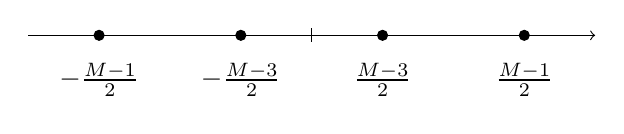
\begin{tikzpicture}[scale=.9]
    \draw[->] (-4,0) -- (4,0);
    \draw[-] (0,.1) -- (0,-.1);
    \draw[fill] (-3,0) circle (2pt);
	    \node[below] at (-3,-.25) {$-\frac{M-1}{2}$};
    \draw[fill] (-1,0) circle (2pt);
	    \node[below] at (-1,-.25) {$-\frac{M-3}{2}$};
	  \draw[fill] (1,0) circle (2pt);
	 	    \node[below] at (1,-.25) {$\frac{M-3}{2}$};
    \draw[fill] (3,0) circle (2pt);
	    \node[below] at (3,-.25) {$\frac{M-1}{2}$};
\end{tikzpicture}
\end{center}

\section{Phasenmodulation (PSK)}
Basisband:
\[
	s(t) = \sum_{k} a_k \cdot p(t-kT_b) 
	\qquad , a_k \in \left\lbrace \e^{\frac{\im 2 \pi 0}{M}}, \e^{\frac{\im 2 \pi 1}{M}}, \ldots,
	\e^{\frac{\im 2 \pi (M-1)}{M}} \right\rbrace
\]
~\\
Bandpasssignal:
\[
	s_{RF}(t) = \Re\lbrace s(t)\rbrace \cos(2\pi f_{RF} t)
		- \Im\lbrace s(t)\rbrace \sin(2\pi f_{RF} t)
\]
~\\
Signalraum:\\
\begin{center}
\begin{tikzpicture}[scale=.9]
   	\draw[->] (-1.5,0) -- (1.5,0) node[below] {\small$Re$};
   	\draw[->] (0,-1.5) -- (0,1.5) node[above right] {\small$Im$};
    \draw[dotted] (0,0) circle (1);	
    \draw[fill] (-1,0) circle (2pt);
    \draw[fill] (-.707,.707) circle (2pt);
    \draw[fill] (0,1) circle (2pt);
    \draw[fill] (.707,.707) circle (2pt);
    \draw[fill] (1,0) circle (2pt);
    \draw[fill] (.707,-.707) circle (2pt);
    \draw[fill] (0,-1) circle (2pt);
    \draw[fill] (-.707,-.707) circle (2pt);
    \node at (2,2) {$\varepsilon_s = 1$};
\end{tikzpicture}
\end{center}

\section{Minimum Shift Keying}
Basisband:
\[\begin{aligned}
	\phi_s(t) = \pi h \left(\sum_{n=-\infty}^{k-1} a_n + a_k \frac{t-kT_s}{T_s} \right)
		\textrm{ mit }
		k=\left\lfloor\frac{t}{T_s}\right\rfloor,\\
		a_k \in \left\lbrace \pm 1, \pm 3,\ldots, \pm (M-1) \right\rbrace
\end{aligned}\]
~\\
Bandpasssignal:
\[
	s_{RF}(t) = \Re\lbrace s(t)\rbrace \cos(2\pi f_{RF} t)
		- \Im\lbrace s(t)\rbrace \sin(2\pi f_{RF} t)
\]

\section{Quadraturamplitudenmodulation (QAM)}
Basisband:
\[
	s(t) = \sum_{k} a_k \cdot p(t-kT_s)
\]
~\\
Bandpasssignal:
\[
	s_{RF}(t) = \Re\lbrace s(t)\rbrace \cos(2\pi f_{RF} t)
		- \Im\lbrace s(t)\rbrace \sin(2\pi f_{RF} t)
\]
~\\
Modulator/Demoudlation:
\begin{center}
	\includegraphics[width=.9\textwidth]{images/qam_modde.jpg}
\end{center}
~\\Bsp: 16-QAM:\\
\begin{center}
\begin{tikzpicture}[scale=.5]
   	\draw[->] (-4,0) -- (4,0) node[below] {\small$I$};
   	\draw[->] (0,-4) -- (0,4) node[above right] {\small$Q$};
    \draw[dotted] (-4,2) -- (4,2);	
    \draw[dotted] (-4,-2) -- (4,-2);    
    \draw[dotted] (-2,-4) -- (-2,4);	
    \draw[dotted] (2,-4) -- (2,4);	
    
    \draw[fill] (-3,3) circle (2pt);
    \draw[fill] (-1,3) circle (2pt);
    \draw[fill] (1,3) circle (2pt);
    \draw[fill] (3,3) circle (2pt);
    
    \draw[fill] (-3,1) circle (2pt);
    \draw[fill] (-1,1) circle (2pt);
    \draw[fill] (1,1) circle (2pt);
    \draw[fill] (3,1) circle (2pt);
    
    \draw[fill] (-3,-1) circle (2pt);
    \draw[fill] (-1,-1) circle (2pt);
    \draw[fill] (1,-1) circle (2pt);
    \draw[fill] (3,-1) circle (2pt);
        
    \draw[fill] (-3,-3) circle (2pt);
    \draw[fill] (-1,-3) circle (2pt);
    \draw[fill] (1,-3) circle (2pt);
    \draw[fill] (3,-3) circle (2pt);
\end{tikzpicture}
\end{center}
